% Options for packages loaded elsewhere
\PassOptionsToPackage{unicode}{hyperref}
\PassOptionsToPackage{hyphens}{url}
%
\documentclass[
]{article}
\usepackage{amsmath,amssymb}
\usepackage{lmodern}
\usepackage{iftex}
\ifPDFTeX
  \usepackage[T1]{fontenc}
  \usepackage[utf8]{inputenc}
  \usepackage{textcomp} % provide euro and other symbols
\else % if luatex or xetex
  \usepackage{unicode-math}
  \defaultfontfeatures{Scale=MatchLowercase}
  \defaultfontfeatures[\rmfamily]{Ligatures=TeX,Scale=1}
\fi
% Use upquote if available, for straight quotes in verbatim environments
\IfFileExists{upquote.sty}{\usepackage{upquote}}{}
\IfFileExists{microtype.sty}{% use microtype if available
  \usepackage[]{microtype}
  \UseMicrotypeSet[protrusion]{basicmath} % disable protrusion for tt fonts
}{}
\makeatletter
\@ifundefined{KOMAClassName}{% if non-KOMA class
  \IfFileExists{parskip.sty}{%
    \usepackage{parskip}
  }{% else
    \setlength{\parindent}{0pt}
    \setlength{\parskip}{6pt plus 2pt minus 1pt}}
}{% if KOMA class
  \KOMAoptions{parskip=half}}
\makeatother
\usepackage{xcolor}
\usepackage[margin=1in]{geometry}
\usepackage{color}
\usepackage{fancyvrb}
\newcommand{\VerbBar}{|}
\newcommand{\VERB}{\Verb[commandchars=\\\{\}]}
\DefineVerbatimEnvironment{Highlighting}{Verbatim}{commandchars=\\\{\}}
% Add ',fontsize=\small' for more characters per line
\usepackage{framed}
\definecolor{shadecolor}{RGB}{248,248,248}
\newenvironment{Shaded}{\begin{snugshade}}{\end{snugshade}}
\newcommand{\AlertTok}[1]{\textcolor[rgb]{0.94,0.16,0.16}{#1}}
\newcommand{\AnnotationTok}[1]{\textcolor[rgb]{0.56,0.35,0.01}{\textbf{\textit{#1}}}}
\newcommand{\AttributeTok}[1]{\textcolor[rgb]{0.77,0.63,0.00}{#1}}
\newcommand{\BaseNTok}[1]{\textcolor[rgb]{0.00,0.00,0.81}{#1}}
\newcommand{\BuiltInTok}[1]{#1}
\newcommand{\CharTok}[1]{\textcolor[rgb]{0.31,0.60,0.02}{#1}}
\newcommand{\CommentTok}[1]{\textcolor[rgb]{0.56,0.35,0.01}{\textit{#1}}}
\newcommand{\CommentVarTok}[1]{\textcolor[rgb]{0.56,0.35,0.01}{\textbf{\textit{#1}}}}
\newcommand{\ConstantTok}[1]{\textcolor[rgb]{0.00,0.00,0.00}{#1}}
\newcommand{\ControlFlowTok}[1]{\textcolor[rgb]{0.13,0.29,0.53}{\textbf{#1}}}
\newcommand{\DataTypeTok}[1]{\textcolor[rgb]{0.13,0.29,0.53}{#1}}
\newcommand{\DecValTok}[1]{\textcolor[rgb]{0.00,0.00,0.81}{#1}}
\newcommand{\DocumentationTok}[1]{\textcolor[rgb]{0.56,0.35,0.01}{\textbf{\textit{#1}}}}
\newcommand{\ErrorTok}[1]{\textcolor[rgb]{0.64,0.00,0.00}{\textbf{#1}}}
\newcommand{\ExtensionTok}[1]{#1}
\newcommand{\FloatTok}[1]{\textcolor[rgb]{0.00,0.00,0.81}{#1}}
\newcommand{\FunctionTok}[1]{\textcolor[rgb]{0.00,0.00,0.00}{#1}}
\newcommand{\ImportTok}[1]{#1}
\newcommand{\InformationTok}[1]{\textcolor[rgb]{0.56,0.35,0.01}{\textbf{\textit{#1}}}}
\newcommand{\KeywordTok}[1]{\textcolor[rgb]{0.13,0.29,0.53}{\textbf{#1}}}
\newcommand{\NormalTok}[1]{#1}
\newcommand{\OperatorTok}[1]{\textcolor[rgb]{0.81,0.36,0.00}{\textbf{#1}}}
\newcommand{\OtherTok}[1]{\textcolor[rgb]{0.56,0.35,0.01}{#1}}
\newcommand{\PreprocessorTok}[1]{\textcolor[rgb]{0.56,0.35,0.01}{\textit{#1}}}
\newcommand{\RegionMarkerTok}[1]{#1}
\newcommand{\SpecialCharTok}[1]{\textcolor[rgb]{0.00,0.00,0.00}{#1}}
\newcommand{\SpecialStringTok}[1]{\textcolor[rgb]{0.31,0.60,0.02}{#1}}
\newcommand{\StringTok}[1]{\textcolor[rgb]{0.31,0.60,0.02}{#1}}
\newcommand{\VariableTok}[1]{\textcolor[rgb]{0.00,0.00,0.00}{#1}}
\newcommand{\VerbatimStringTok}[1]{\textcolor[rgb]{0.31,0.60,0.02}{#1}}
\newcommand{\WarningTok}[1]{\textcolor[rgb]{0.56,0.35,0.01}{\textbf{\textit{#1}}}}
\usepackage{graphicx}
\makeatletter
\def\maxwidth{\ifdim\Gin@nat@width>\linewidth\linewidth\else\Gin@nat@width\fi}
\def\maxheight{\ifdim\Gin@nat@height>\textheight\textheight\else\Gin@nat@height\fi}
\makeatother
% Scale images if necessary, so that they will not overflow the page
% margins by default, and it is still possible to overwrite the defaults
% using explicit options in \includegraphics[width, height, ...]{}
\setkeys{Gin}{width=\maxwidth,height=\maxheight,keepaspectratio}
% Set default figure placement to htbp
\makeatletter
\def\fps@figure{htbp}
\makeatother
\setlength{\emergencystretch}{3em} % prevent overfull lines
\providecommand{\tightlist}{%
  \setlength{\itemsep}{0pt}\setlength{\parskip}{0pt}}
\setcounter{secnumdepth}{-\maxdimen} % remove section numbering
\usepackage{booktabs}
\usepackage{longtable}
\usepackage{array}
\usepackage{multirow}
\usepackage{wrapfig}
\usepackage{float}
\usepackage{colortbl}
\usepackage{pdflscape}
\usepackage{tabu}
\usepackage{threeparttable}
\usepackage{threeparttablex}
\usepackage[normalem]{ulem}
\usepackage{makecell}
\usepackage{xcolor}
\usepackage{amsmath}
\usepackage{caption}
\ifLuaTeX
  \usepackage{selnolig}  % disable illegal ligatures
\fi
\IfFileExists{bookmark.sty}{\usepackage{bookmark}}{\usepackage{hyperref}}
\IfFileExists{xurl.sty}{\usepackage{xurl}}{} % add URL line breaks if available
\urlstyle{same} % disable monospaced font for URLs
\hypersetup{
  pdftitle={A07 - Crafting Reports},
  pdfauthor={Griffin Bird},
  hidelinks,
  pdfcreator={LaTeX via pandoc}}

\title{A07 - Crafting Reports}
\author{Griffin Bird}
\date{Spring 2023}

\begin{document}
\maketitle

\hypertarget{objectives}{%
\subsection{Objectives:}\label{objectives}}

\begin{enumerate}
\def\labelenumi{\arabic{enumi}.}
\tightlist
\item
  More practice with R code chunk options
\item
  Gain proficiency with figures, tables (w/\texttt{Kable}) table of
  contents, etc.
\item
  Debugging knitting issues
\end{enumerate}

\hypertarget{directions}{%
\subsection{Directions}\label{directions}}

\begin{enumerate}
\def\labelenumi{\arabic{enumi}.}
\tightlist
\item
  Rename this file
  \texttt{\textless{}FirstLast\textgreater{}\_A07\_CraftingReports.Rmd}
  (replacing \texttt{\textless{}FirstLast\textgreater{}} with your first
  and last name).
\item
  Change ``Student Name'' on line 3 (above) with your name.
\item
  Work through the tasks, \textbf{creating code and output} that fulfill
  each instruction.
\item
  Be sure your code is tidy; use line breaks to ensure your code fits in
  the knitted output.
\item
  Be sure to \textbf{answer the questions} in this assignment document.
\item
  When you have completed the assignment, \textbf{Knit} the text and
  code into a single PDF file.
\item
  \textbf{Be sure that you also commit and push your final Rmd document
  to your GitHub account}.
\end{enumerate}

\hypertarget{task-1---basic-markdown}{%
\subsection{Task 1 - Basic Markdown}\label{task-1---basic-markdown}}

Create a table below summarizing the metadata of the EPA Air Quality
data. The first column will be the metadata attribute item name:
``Source'', ``Date'', and ``Filename''. And the second column will
include the metadata values: ``EPA Air Quality SYstem (AQS)'',
``2018-2019'', and ``EPAair\_O3\_PM25\_NC1819\_Processed.csv''. The
first column should be aligned to the right and the second to the left.

\begin{Shaded}
\begin{Highlighting}[]
\FunctionTok{library}\NormalTok{(tidyverse)}
\FunctionTok{library}\NormalTok{(agricolae)}
\FunctionTok{library}\NormalTok{(here)}
\FunctionTok{library}\NormalTok{(ggplot2)}
\FunctionTok{library}\NormalTok{(ggthemes)}
\FunctionTok{library}\NormalTok{(dplyr)}
\FunctionTok{library}\NormalTok{(lubridate)}
\FunctionTok{library}\NormalTok{(knitr)}
\FunctionTok{library}\NormalTok{(dplyr)}
\FunctionTok{library}\NormalTok{(gt)}
\FunctionTok{library}\NormalTok{(kableExtra)}
\FunctionTok{library}\NormalTok{(tinytex)}

\NormalTok{knitr}\SpecialCharTok{::}\NormalTok{opts\_chunk}\SpecialCharTok{$}\FunctionTok{set}\NormalTok{(}\AttributeTok{tidy.opts=}\FunctionTok{list}\NormalTok{(}\AttributeTok{width.cutoff=}\DecValTok{80}\NormalTok{), }\AttributeTok{tidy=}\ConstantTok{TRUE}\NormalTok{)}

\FunctionTok{here}\NormalTok{()}
\end{Highlighting}
\end{Shaded}

\begin{Shaded}
\begin{Highlighting}[]
\NormalTok{AirQuality }\OtherTok{\textless{}{-}} \FunctionTok{read.csv}\NormalTok{(}\StringTok{"C:/Users/17038/Documents/EDASpring2023/Data/Processed/EPAair\_O3\_PM25\_NC1819\_Processed.csv"}\NormalTok{)}

\NormalTok{Metadata }\OtherTok{\textless{}{-}} \FunctionTok{data.frame}\NormalTok{(}\StringTok{\textasciigrave{}}\AttributeTok{Metadata Attributes}\StringTok{\textasciigrave{}} \OtherTok{=} \FunctionTok{rep}\NormalTok{(}\FunctionTok{c}\NormalTok{(}\StringTok{"Source"}\NormalTok{, }\StringTok{"Date"}\NormalTok{, }\StringTok{"Filename"}\NormalTok{)),}
    \AttributeTok{Values =} \FunctionTok{rep}\NormalTok{(}\FunctionTok{c}\NormalTok{(}\StringTok{"EPA Air Quality SYstem (AQS)"}\NormalTok{, }\StringTok{"2018{-}2019"}\NormalTok{, }\StringTok{"EPAair\_O3\_PM25\_NC1819\_Processed.csv"}\NormalTok{)))}

\NormalTok{Metadata }\SpecialCharTok{\%\textgreater{}\%}
    \FunctionTok{gt}\NormalTok{() }\SpecialCharTok{\%\textgreater{}\%}
    \FunctionTok{cols\_align}\NormalTok{(}\AttributeTok{align =} \StringTok{"right"}\NormalTok{, }\AttributeTok{columns =}\NormalTok{ Metadata.Attributes) }\SpecialCharTok{\%\textgreater{}\%}
    \FunctionTok{cols\_align}\NormalTok{(}\AttributeTok{align =} \StringTok{"left"}\NormalTok{, }\AttributeTok{columns =}\NormalTok{ Values)}
\end{Highlighting}
\end{Shaded}

\begin{longtable}{rl}
\toprule
Metadata.Attributes & Values \\ 
\midrule
Source & EPA Air Quality SYstem (AQS) \\ 
Date & 2018-2019 \\ 
Filename & EPAair\_O3\_PM25\_NC1819\_Processed.csv \\ 
\bottomrule
\end{longtable}

\begin{center}\rule{0.5\linewidth}{0.5pt}\end{center}

\hypertarget{task-2---import-packages-and-data-suppressing-messages}{%
\subsection{Task 2 - Import packages and data, suppressing
messages}\label{task-2---import-packages-and-data-suppressing-messages}}

Set the following R code chunk so that it runs when knit, but no
messages, errors, or any output is shown. The code itself should be
displayed.

\begin{Shaded}
\begin{Highlighting}[]
\CommentTok{\# Import libraries}
\FunctionTok{library}\NormalTok{(tidyverse)}
\FunctionTok{library}\NormalTok{(lubridate)}
\FunctionTok{library}\NormalTok{(here)}
\FunctionTok{library}\NormalTok{(knitr)}

\CommentTok{\# Import EPA data (from the processed\_KEY folder) \& fix dates}
\NormalTok{epa\_data }\OtherTok{\textless{}{-}} \FunctionTok{read.csv}\NormalTok{(}\FunctionTok{here}\NormalTok{(}\StringTok{"data"}\NormalTok{, }\StringTok{"processed\_KEY"}\NormalTok{, }\StringTok{"EPAair\_O3\_PM25\_NC1819\_Processed.csv"}\NormalTok{),}
    \AttributeTok{stringsAsFactors =} \ConstantTok{TRUE}\NormalTok{) }\SpecialCharTok{\%\textgreater{}\%}
    \FunctionTok{mutate}\NormalTok{(}\AttributeTok{Date =} \FunctionTok{ymd}\NormalTok{(Date))}
\end{Highlighting}
\end{Shaded}

\begin{center}\rule{0.5\linewidth}{0.5pt}\end{center}

\hypertarget{task-3-creating-tables}{%
\subsection{Task 3: Creating tables}\label{task-3-creating-tables}}

Set the following R code chunk to display two tables, using knitr's
\texttt{kable()} function, one listing the mean PM2.5 concentrations for
each county, and the other the same except for Ozone. The titles should
be ``Mean Particulates (2.5mm)'' and ``Mean Ozone'', respectively. And
the column names should be ``County'' and ``µg/m3'' for both tables.

Customize the chunk options such that the code is run but is not
displayed in the knitted document. The output, however, should be
displayed.

\begin{quote}
\textbf{TIPS:}

\begin{itemize}
\item
  Use \texttt{"\$\textbackslash{}\textbackslash{}mu\ g/m\^{}3\$"} as a
  column name to generate a nicely formatted string via markdown/MathJax
  notation
\item
  If your output table spans across two pages, try inserting a new line
  (via \texttt{\textbackslash{}newpage}) in the markdown just before
  your code chunk.
\end{itemize}
\end{quote}

\begin{table}

\caption{\label{tab:data.summary}Mean Particulates (2.5mm)}
\centering
\begin{tabular}[t]{l|r}
\hline
County & \$\textbackslash{}mu g/m\textasciicircum{}3\$\\
\hline
Haywood & 13.98400\\
\hline
New Hanover & 15.60681\\
\hline
Avery & 18.27941\\
\hline
Edgecombe & 26.06503\\
\hline
Pitt & 27.37166\\
\hline
Guilford & 29.14163\\
\hline
Swain & 30.62780\\
\hline
Johnston & 33.02695\\
\hline
Durham & 33.53770\\
\hline
Mecklenburg & 33.63038\\
\hline
Forsyth & 35.09282\\
\hline
Wake & 37.45423\\
\hline
\end{tabular}
\end{table}

\begin{table}

\caption{\label{tab:data.summary}Mean Ozone}
\centering
\begin{tabular}[t]{l|r}
\hline
County & \$\textbackslash{}mu g/m\textasciicircum{}3\$\\
\hline
Swain & 35.58367\\
\hline
Avery & 38.39308\\
\hline
Wake & 38.61345\\
\hline
New Hanover & 39.11688\\
\hline
Edgecombe & 39.22154\\
\hline
Johnston & 40.33849\\
\hline
Mecklenburg & 40.45746\\
\hline
Durham & 40.69882\\
\hline
Pitt & 41.64147\\
\hline
Forsyth & 44.02352\\
\hline
Haywood & 44.75049\\
\hline
Guilford & 45.86681\\
\hline
\end{tabular}
\end{table}

\newpage

\hypertarget{task-3-plots}{%
\subsection{Task 3: Plots}\label{task-3-plots}}

Create two separate code chunks that create boxplots of the distribution
of Ozone levels by month using, one for only records collected in 2018
and one for records in 2019. Customize the chunk options such that the
final figures are displayed but not the code used to generate the
figures. In addition, the plots aligned on the left side of the page and
set the figure heights so both plots fit on the same page with minimal
space remaining. Lastly, add a \texttt{fig.cap} chunk option to add a
caption (title) to your plot that will display underneath the figure.

\begin{figure}

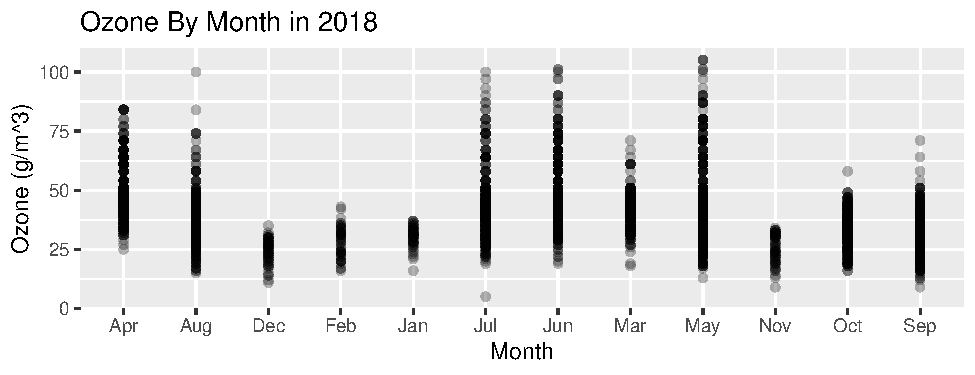
\includegraphics{GriffinBird_A07_Lab_Crafting_Reports_files/figure-latex/Ozone2018-1} \hfill{}

\caption{Ozone Levels by Month 2018}\label{fig:Ozone2018}
\end{figure}

\begin{figure}

\hfill{}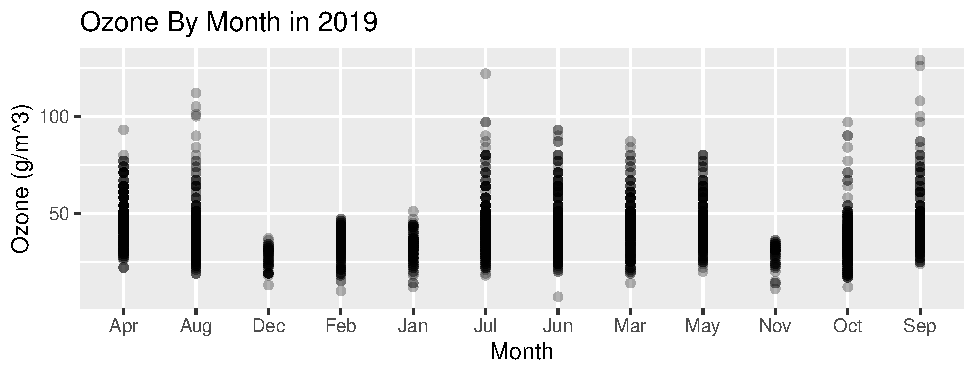
\includegraphics{GriffinBird_A07_Lab_Crafting_Reports_files/figure-latex/Ozone2019-1} 

\caption{Ozone Levels by Month 2019}\label{fig:Ozone2019}
\end{figure}

\newpage

\hypertarget{task-4-knit-and-submit.}{%
\subsection{Task 4: Knit and submit.}\label{task-4-knit-and-submit.}}

Add a table of contents to your document and knit to a PDF. Submit your
PDF to Sakai, but also be sure to commit and push your Rmd file used to
create this knit document to GitHub. In the section below, add a link to
your GitHub repository.

\hypertarget{git-repository}{%
\subsubsection{Git Repository}\label{git-repository}}

\url{https://github.com/griff0523/EDA-Spring2023}

\end{document}
